\documentclass{main.tex}[subfiles]
\begin{document}
\section{Задача распознавания символов Брайля}
\subsection{Общая постановка задачи и особенности рельефно-точечного шрифта}
\begin{figure}[H]
    \centering
    \begin{subfigure}{.5\textwidth}
        \centering
        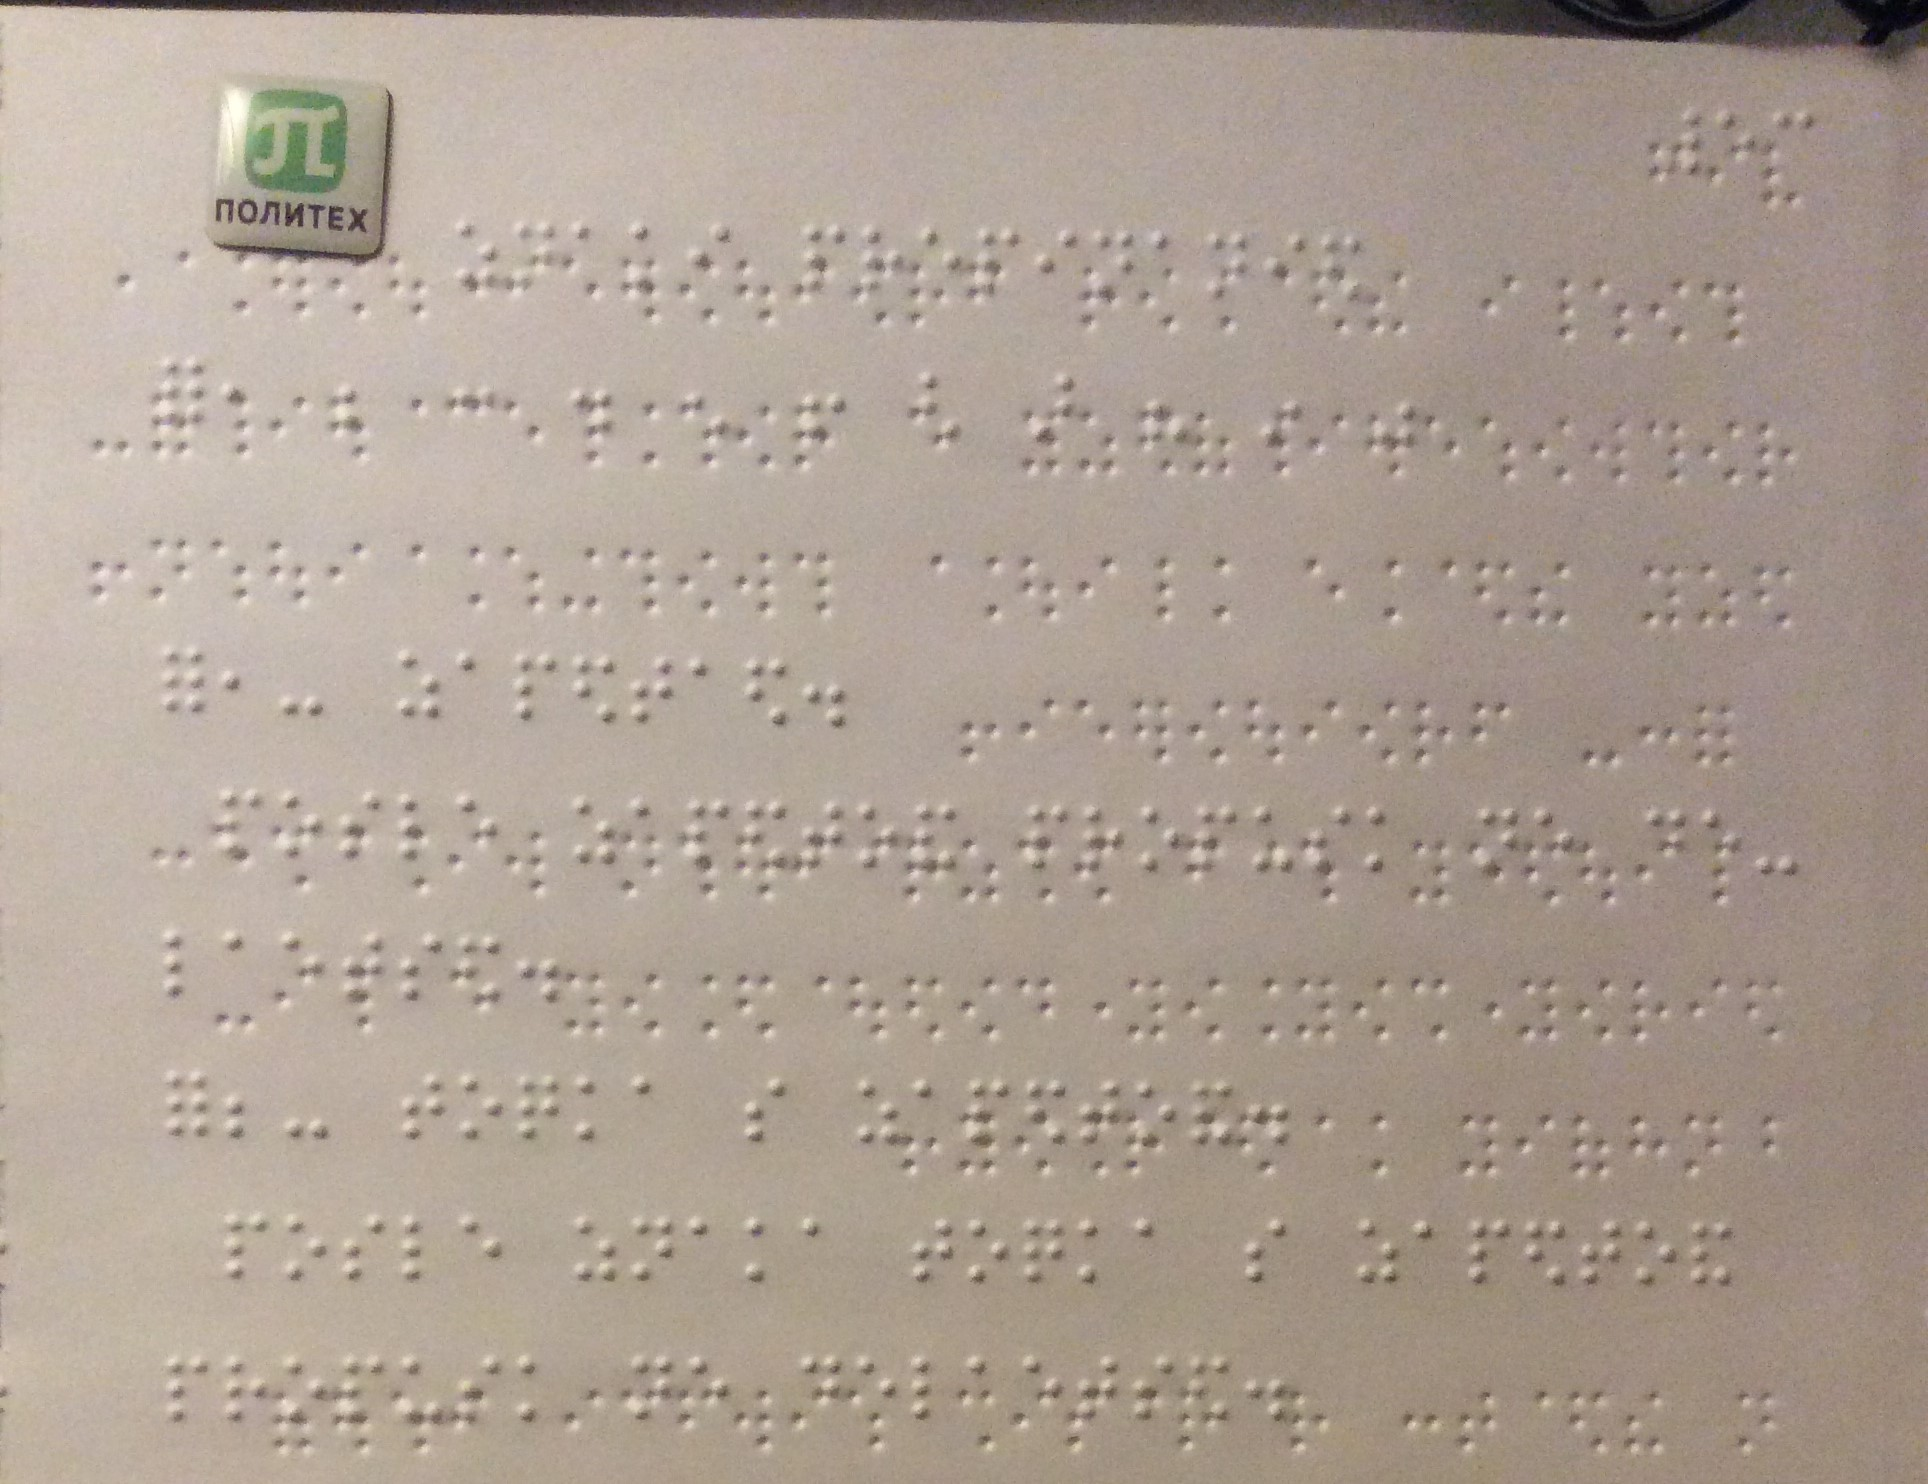
\includegraphics[width=.9\myPictWidth]{brl_book_golubina}
        \caption{книга}
        % TODO \label{fig:}
    \end{subfigure}%
    \begin{subfigure}{.5\textwidth}
        \centering
        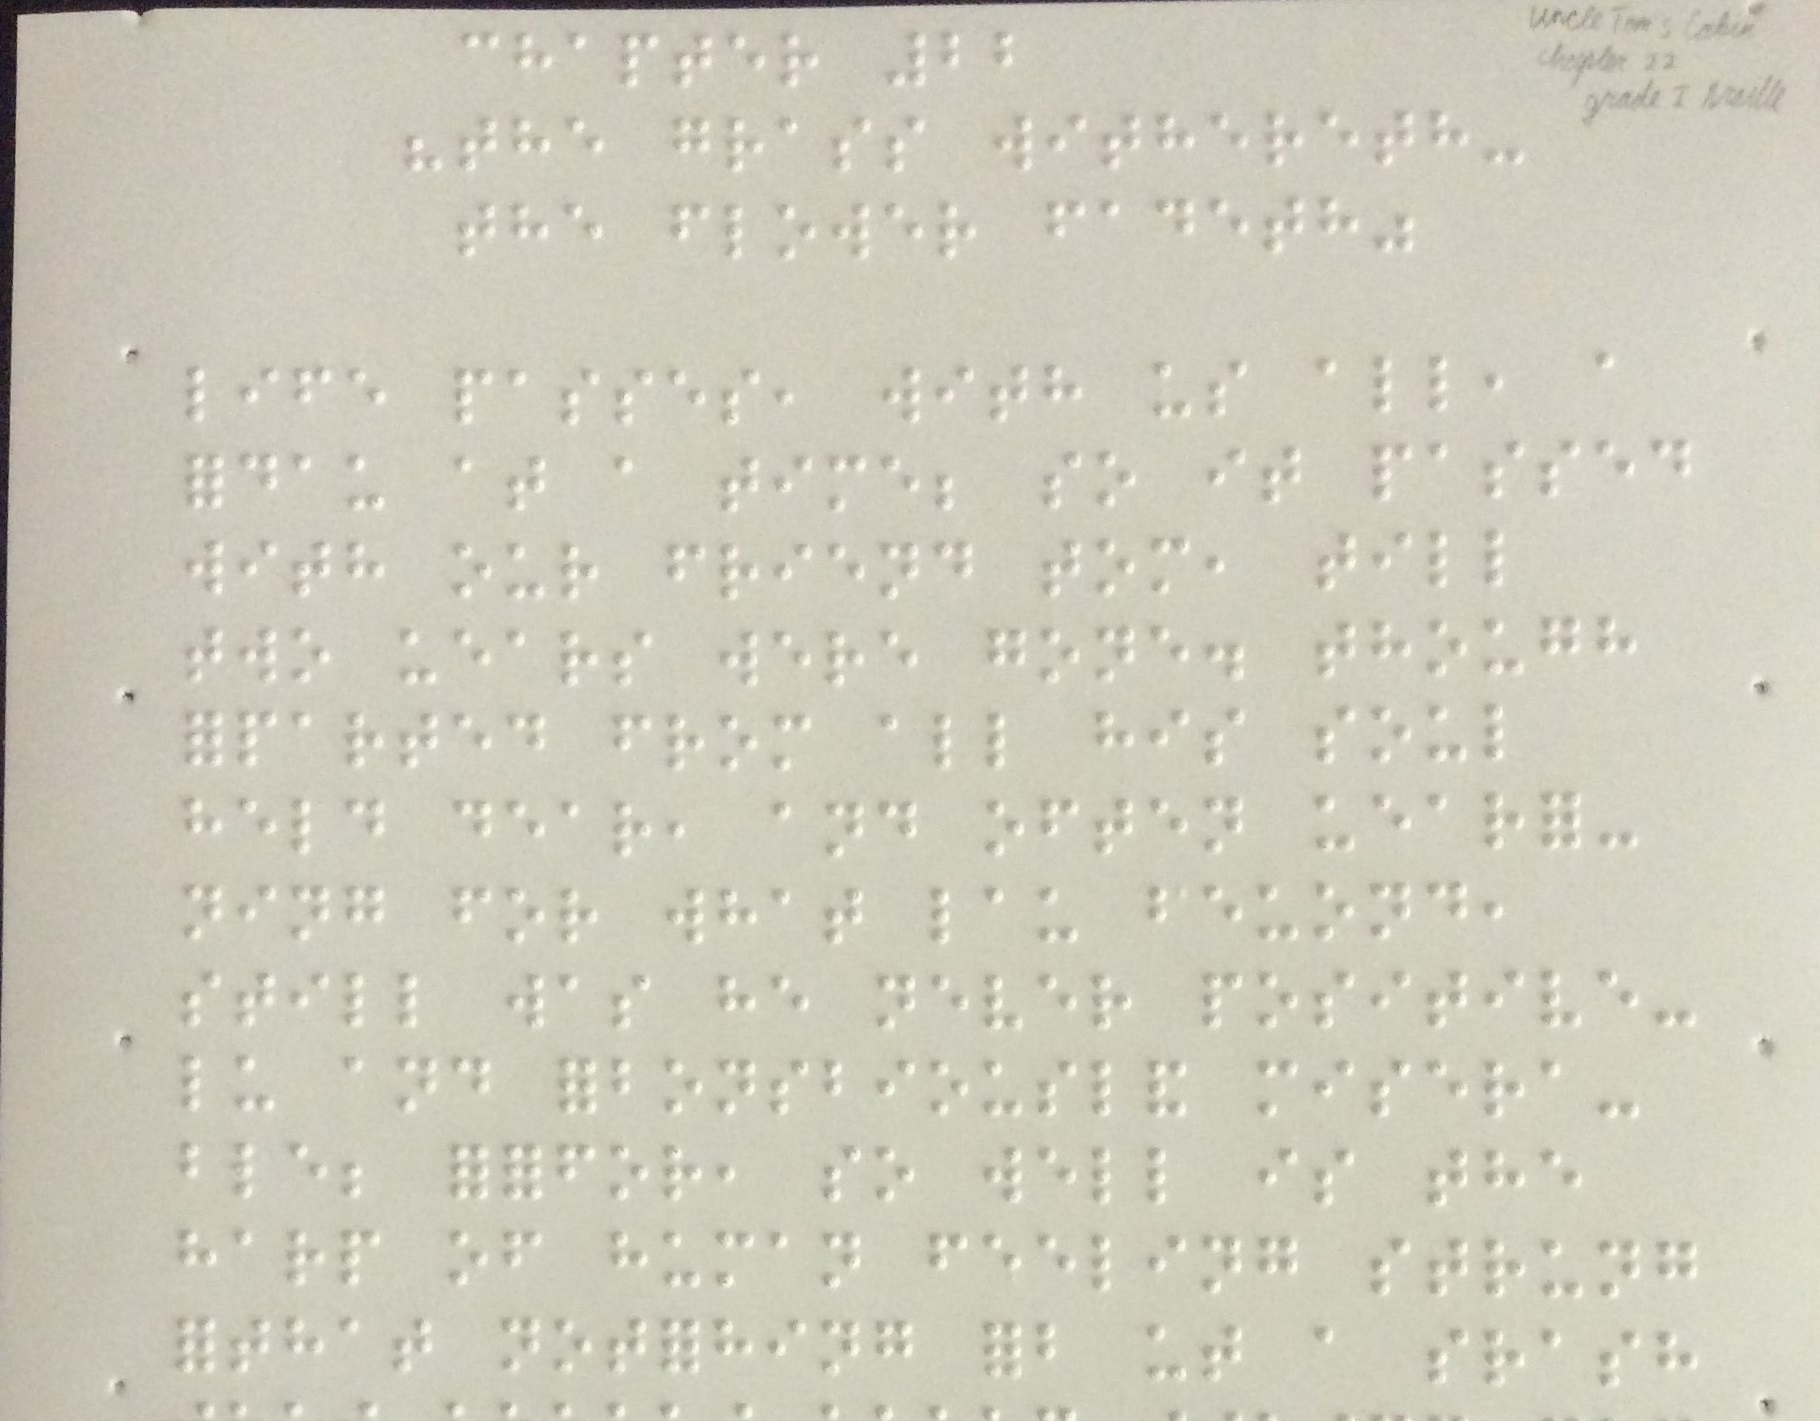
\includegraphics[width=.9\myPictWidth]{brl_writing_uncle_tom}
        \caption{рукопись}
        % TODO \label{fig:}
    \end{subfigure}
    \caption{Листы с рельефно-точечным шрифтом Брайля}
    \label{fig:brl_example} % TODO ref in the text
\end{figure}
\subsection{Обзор существующих решений}
\subsubsection{Подходы к распознаванию}

\cite{baumgartner2020app}
\cite{li2020braunet}
\cite{ovodov2020}
\cite{ovodov2021}
\cite{alsalman2021}
\cite{ortoncelli2021}

\subsubsection{Наборы данных}

\subsection{Цели и задачи настоящей работы}

\end{document}
